\documentclass[12pt]{exam}
\pagestyle{headandfoot}
\firstpageheader{}{}{}
\runningheader{\date}{}{\class, \teacher}
\runningheadrule
\firstpagefooter{}{}{}
\runningfooter{}{Viel Erfolg!}{Seite \thepage\:von \numpages}
\runningfootrule
%=========================================================
\newcommand{\thema}{Geometrie \uproman{2}}
\newcommand{\lehrer}{Jonas Guler}
\newcommand{\klasse}{1GaMa}
\newcommand{\serie}{A}
\newcommand{\data}{\today}
\newcommand{\dauer}{45 Minuten}
\newcommand{\name}{\bf Name:}
\newcommand{\nota}{Note:}
\newcommand{\datum}{02.03.22}
%=========================================================
\begin{document}
\fontsize{14}{14}\selectfont
%========================================================

%========================================================
\begin{tabular*}{\textwidth}{l @{\extracolsep{\fill}}l @{\extracolsep{6pt}}l}
\textbf{\thema} & \textbf{\nota} & {\answerbox}\\
\textbf{Klasse \klasse} & & \\
\textbf{\lehrer}  & {\name} &\textbf{\hrulefill}\\[8pt]
%-------------------
\end{tabular*}
%--------------------
\begin{center}
\rule[1ex]{\textwidth}{1pt}
Dauer: \dauer \hspace{9cm}Datum: \datum\\
\vspace{5pt}
\rule[2ex]{\textwidth}{1pt}
\end{center}
%=========================================================

%=========================================================
\begin{center}
\textbf{Bewertungstabelle}\\
\small Wird von der Lehrperson ausgefüllt\\
\vspace{5pt}
\addpoints
\gradetable[h][questions]\\
\vspace{15pt}
Der Rechenweg muss \textbf{vollständig und nachvollziehbar} sein.\\
Lösen Sie die Prüfung mit einen schwarzen oder blauen Kugelschreiber. Resultate in Bleistift, roter oder grüner Farbe werden nicht berücksichtigt; ausgenommen sind geometrische Konstruktionen.\\
Die Schlussresultate sind auf drei Nachkommastellen zu runden oder vollständig gekürzt anzugeben.\\
Als Hilfsmittel sind nur Zirkel, Geodreieck und Lineal erlaubt.
\end{center}

\noindent
\rule[1ex]{\textwidth}{1pt}

\vspace{10cm}
\begin{center}
    %\Huge{Serie \serie}
\end{center}

\newpage

\begin{questions}
%=========================================================
%---------------------TESTFRAGEN
%=========================================================
\question[4]
\begin{parts}
    \part Erkläre in eigenen Worten den mathematischen Begriff der \flqq Kongruenz\frqq.
\end{parts}
\vspace{5pt}
\antwort{5}
\begin{parts}
    \setcounter{partno}{1}
    \part Erkläre in eigenen Worten die beiden zentralen Punkte, die der Kongruenzsatz \flqq SWS\frqq\:aussagt.
\end{parts}
\vspace{5pt}
\antwort{5}

%---------------------------------------------------------
\newpage
\question[6]
\begin{parts}
    \part Ist das Dreieck $\vartriangle$$ABC$ eindeutig konstruierbar? Begründe deine Antwort.
    \[a=6\text{cm},\:\beta=36^\circ,\:\gamma=48^\circ\]
\end{parts}
\vspace{5pt}
\antwort{4}
\begin{parts}
    \setcounter{partno}{1}
    \part  Begründe, warum das folgende Dreieck nicht eindeutig konstruierbar ist.
    \[b=3\text{cm},\:c=5\text{cm},\beta=39^\circ\]
\end{parts}
\vspace{5pt}
\antwort{6}
\begin{parts}
    \setcounter{partno}{2}
    \part Kann man aus den Angaben schliessen, dass die Dreiecke $\vartriangle$$ABC$ und $\vartriangle$$DEF$ kongruent sind? Gib jeweils den Kongruenzsatz in deiner Argumentation an.
    \[a=3\text{cm},\:\beta=50^\circ,\:\gamma=66^\circ \text{ und } e=3\text{cm},\:\delta=50^\circ,\:\eta=64^\circ\]
    \textbf{Tipp:} $\eta$ ist der Winkel, der Seite $e$ gegenüber liegt.
\end{parts}
\vspace{5pt}
\antwort{6}

%---------------------------------------------------------
\newpage
\question[6]
In der untenstehenden Figur gilt: $\alpha=\beta$ und $\overline{FI}=\overline{IA}$.\\
Beweise, dass die Gerade $TI$ die Winkelhalbierende des Winkels $\vartriangle$$FTA$ ist.
\begin{center}
    
\includegraphics[scale=0.8]{Geometrie/data-geometrie/Kongruenzbeweis-GaMa.png}
\end{center}

\vspace{5pt}
\antwort{16}

%---------------------------------------------------------
\newpage
\question[4]
\begin{parts}
    \part Erkläre in eigenen Worten die mathematische Definition einer \flqq Kongruenzabbildung\frqq.
\end{parts}
\vspace{5pt}
\antwort{6}
\begin{parts}
    \setcounter{partno}{1}
    \part Gib die drei speziellen Eigenschaften der Kongruenzabbildungen an und erläutere jede in maximal einem Satz.
\end{parts}
\vspace{5pt}
\antwort{10}


%---------------------------------------------------------
\newpage
\question[4]
Das Dreieck $ABC$ wird mittels einer Drehung auf das Dreieck $A'B'C'$ abgebildet. Bestimme den Drehpunkt $Z$ und den Drehwinkel $\alpha$.
\vspace{2cm}
\begin{center}
    
\includegraphics[scale=1]{Geometrie/data-geometrie/FindeDrehzentrum.png}
\end{center}
\vfill
\antwort{5}

%---------------------------------------------------------
\newpage
\question[6]
Gegeben sind die Punkte $A=(2,1)$ und $A''=(6,5)$ sowie die Spiegelachse $a_1$, die in $C=(3,0)$ senkrecht auf der x-Achse steht. $A$ wird durch eine Doppelspiegelung $A\xrightarrow{S_{a_1}}A'\xrightarrow{S_{a_2}}A''$ abgebildet.
\begin{parts}
    \part Konstruiere die zweite Spiegelachse $a_2$.
    \part Zeige rechnerisch, dass diese Doppelspiegelung von $A$ auf $A''$ als eine Drehung mit Drehpunkt als Schnittpunkt der beiden Spiegelachsen aufgefasst werden kann.
\end{parts}

\begin{center}
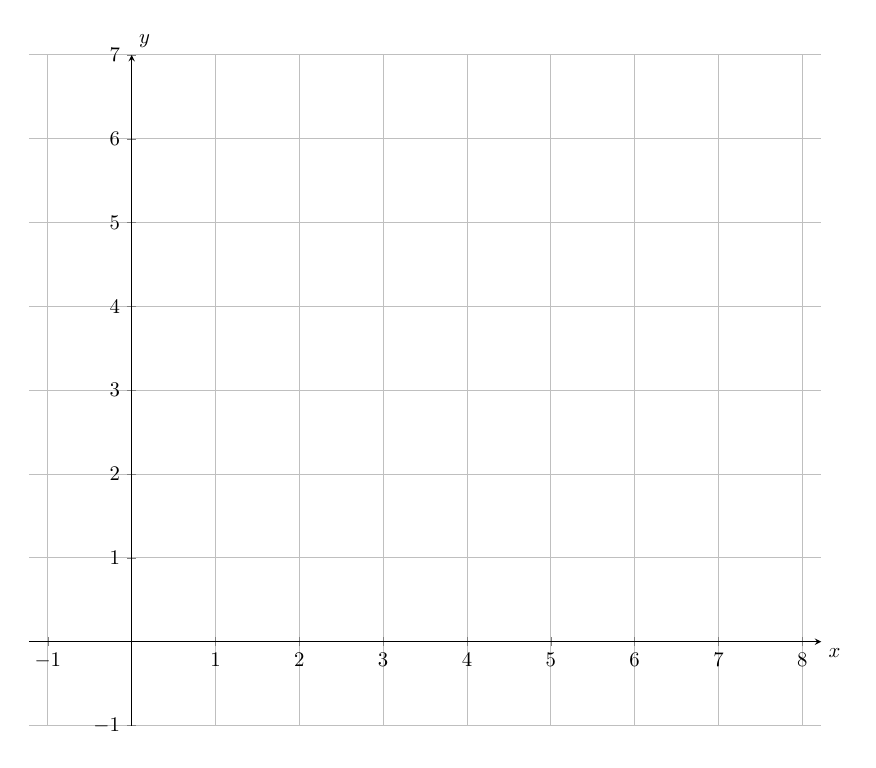
\begin{tikzpicture}[baseline,scale=0.75]
\begin{axis}[
axis y line=center,
axis x line=middle,
axis equal,
grid=major,
xmin=-1,xmax=8,
ymin=-1,ymax=7,
xlabel=$x$,ylabel=$y$,
xlabel style={at={(ticklabel* cs:1)},anchor=north west},
ylabel style={at={(ticklabel* cs:1)},anchor=south west},
xtick={-10,-9,...,10},
ytick={-10,-9,...,10},
width=15cm,
anchor=center,
]
\end{axis}
\end{tikzpicture}
\end{center}
\vfill
\antwort{7}


\end{questions}
\end{document}